\section{Sistema D – Sistema de Segurança}

Quando o sensor PIR deteta movimento fica `suspenso' durante um certo tempo em que não deteta qual movimento. Terminando este intervalo, o sensor está `ativo' novamente pelo que pode ocorrer uma repetição da sinalização de `Alarm On', caso o alarme não seja desarmado nesse meio tempo. No entanto, isto não acontece - como pode verificar no vídeo em anexo - é feita uma verificação para caso o alarme já esteja ativo.

Também é verdade para o desarme do alarme com o pressionar do botão. Múltiplos pressionares não desarmam múltiplas vezes o alarme.

\begin{figure}[H]
    \centering
    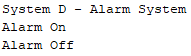
\includegraphics{images/testes/sisD_serialmonitor.png}
    \selectlanguage{portuguese}\caption{Serial Monitor}
\end{figure}

\begin{figure}[H]
    \centering
    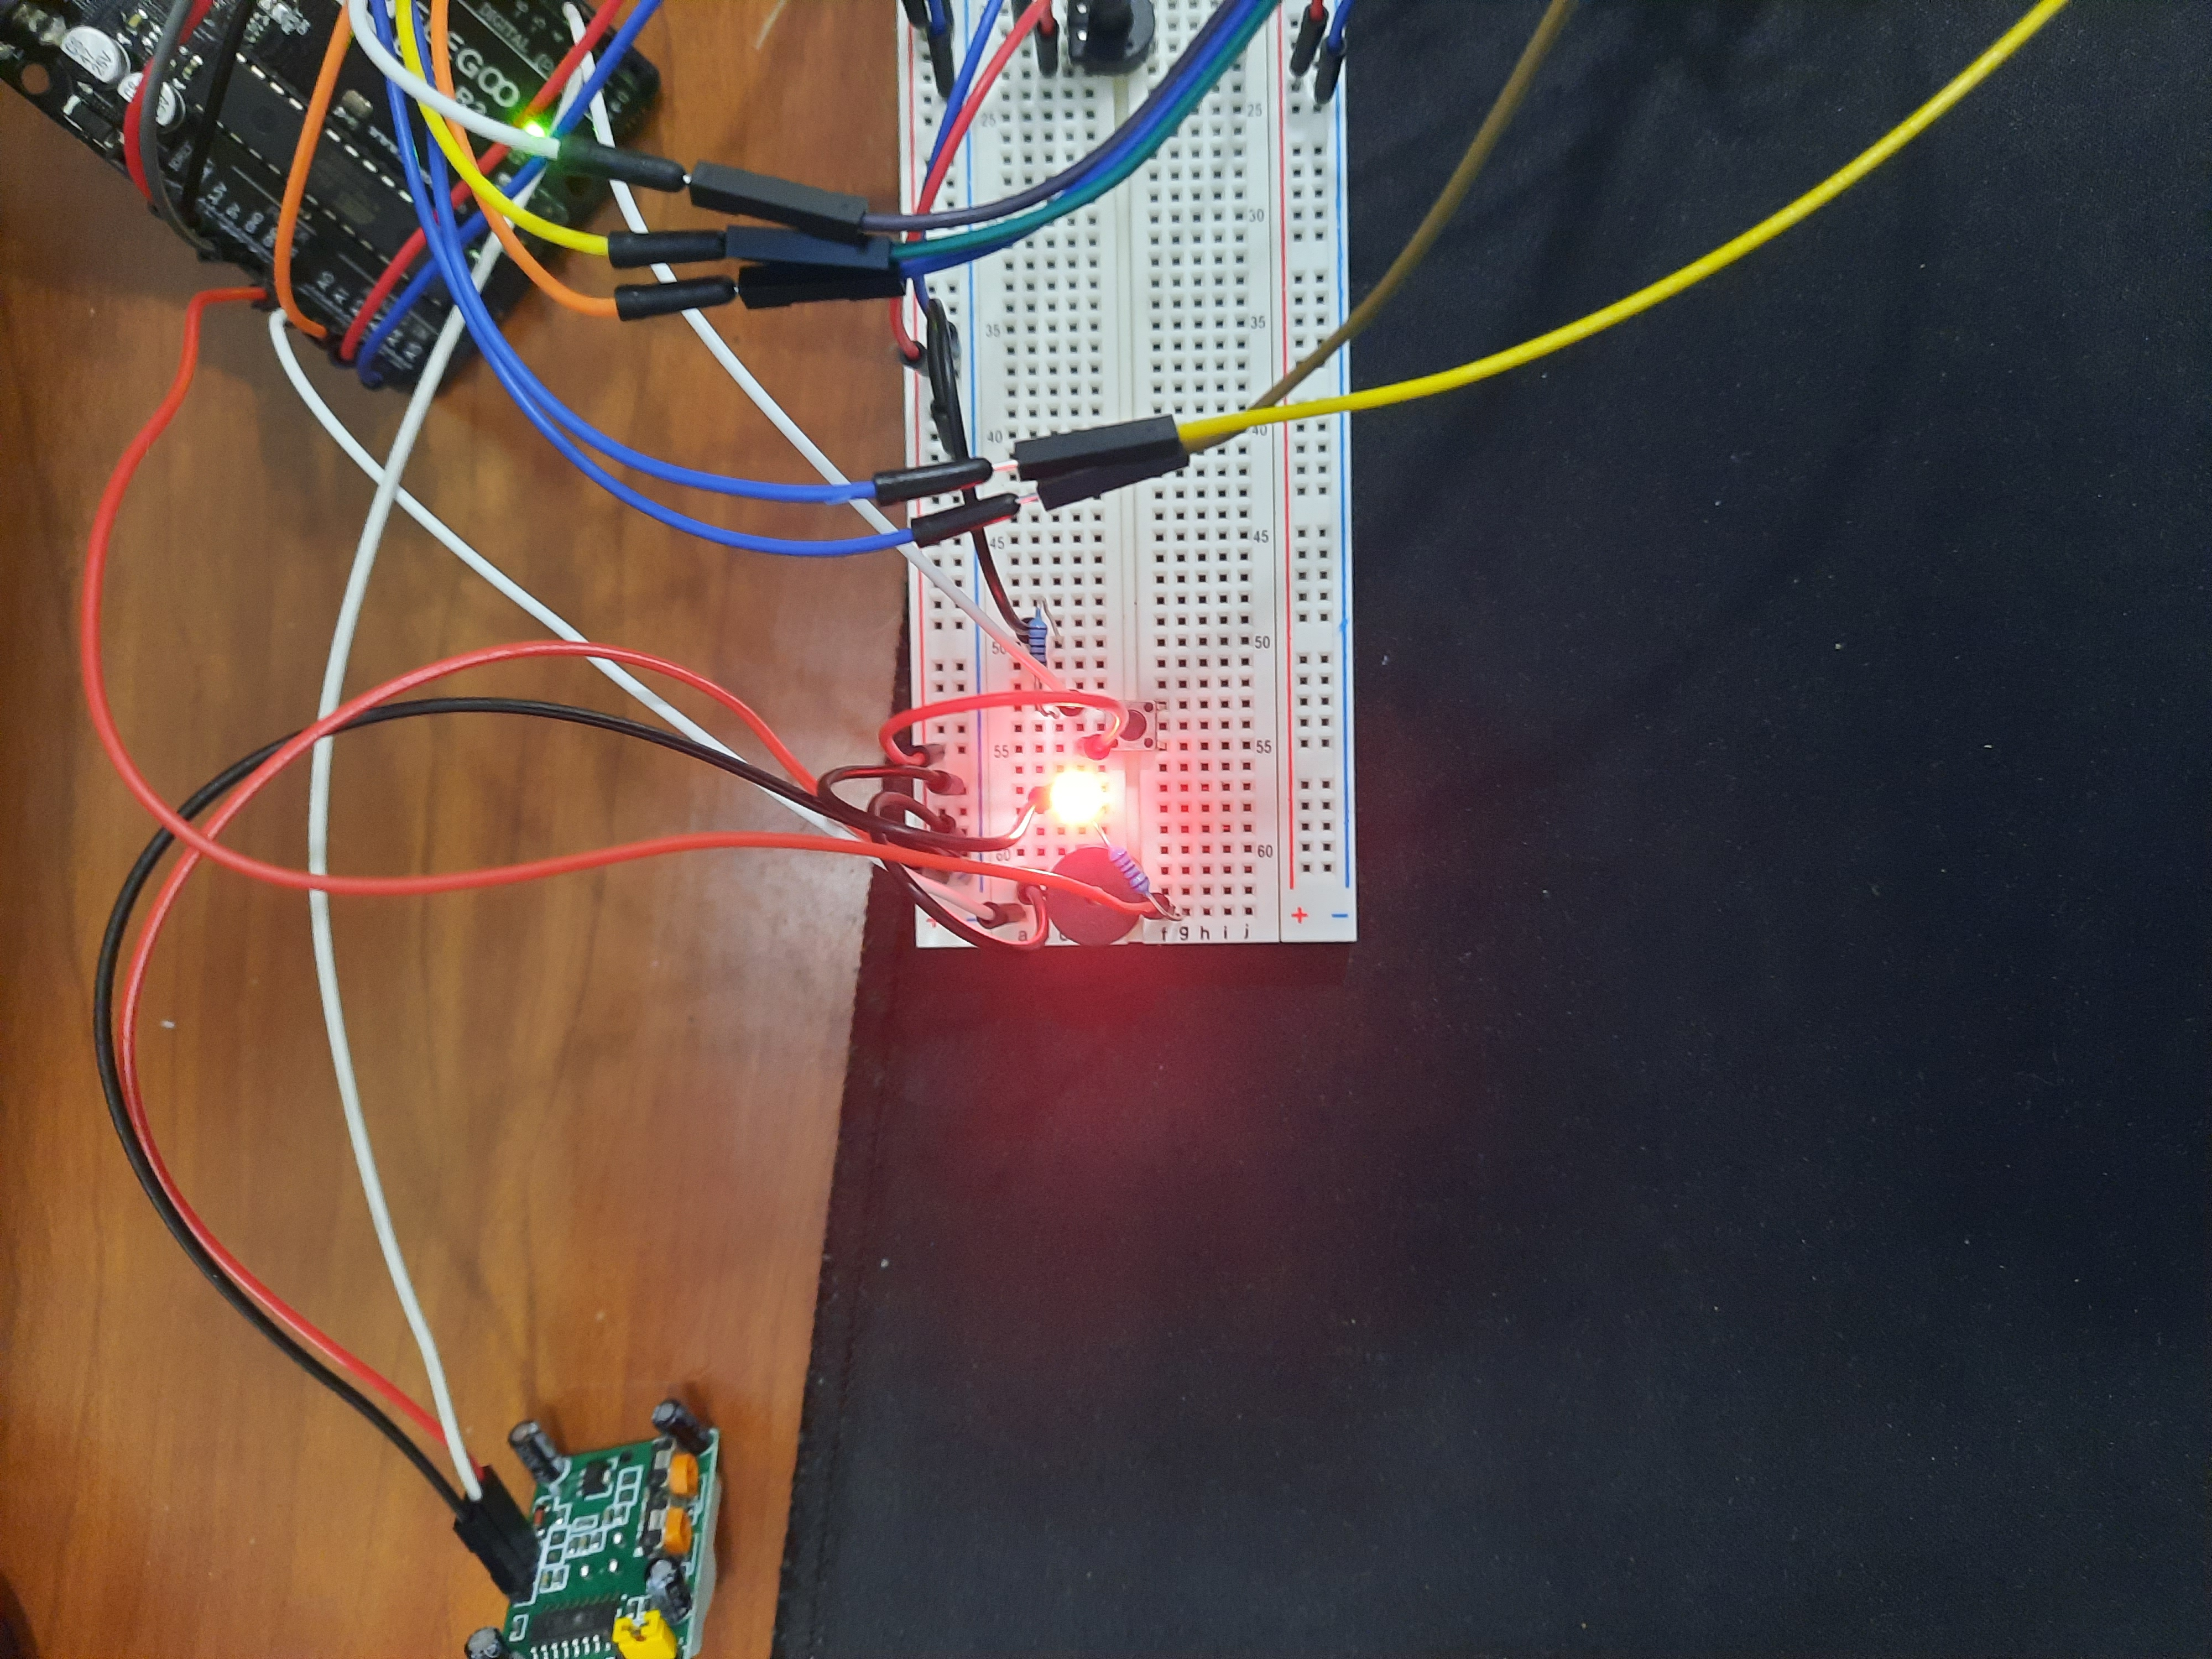
\includegraphics[scale=0.05,angle=-90]{images/testes/sisD_on.jpg}
    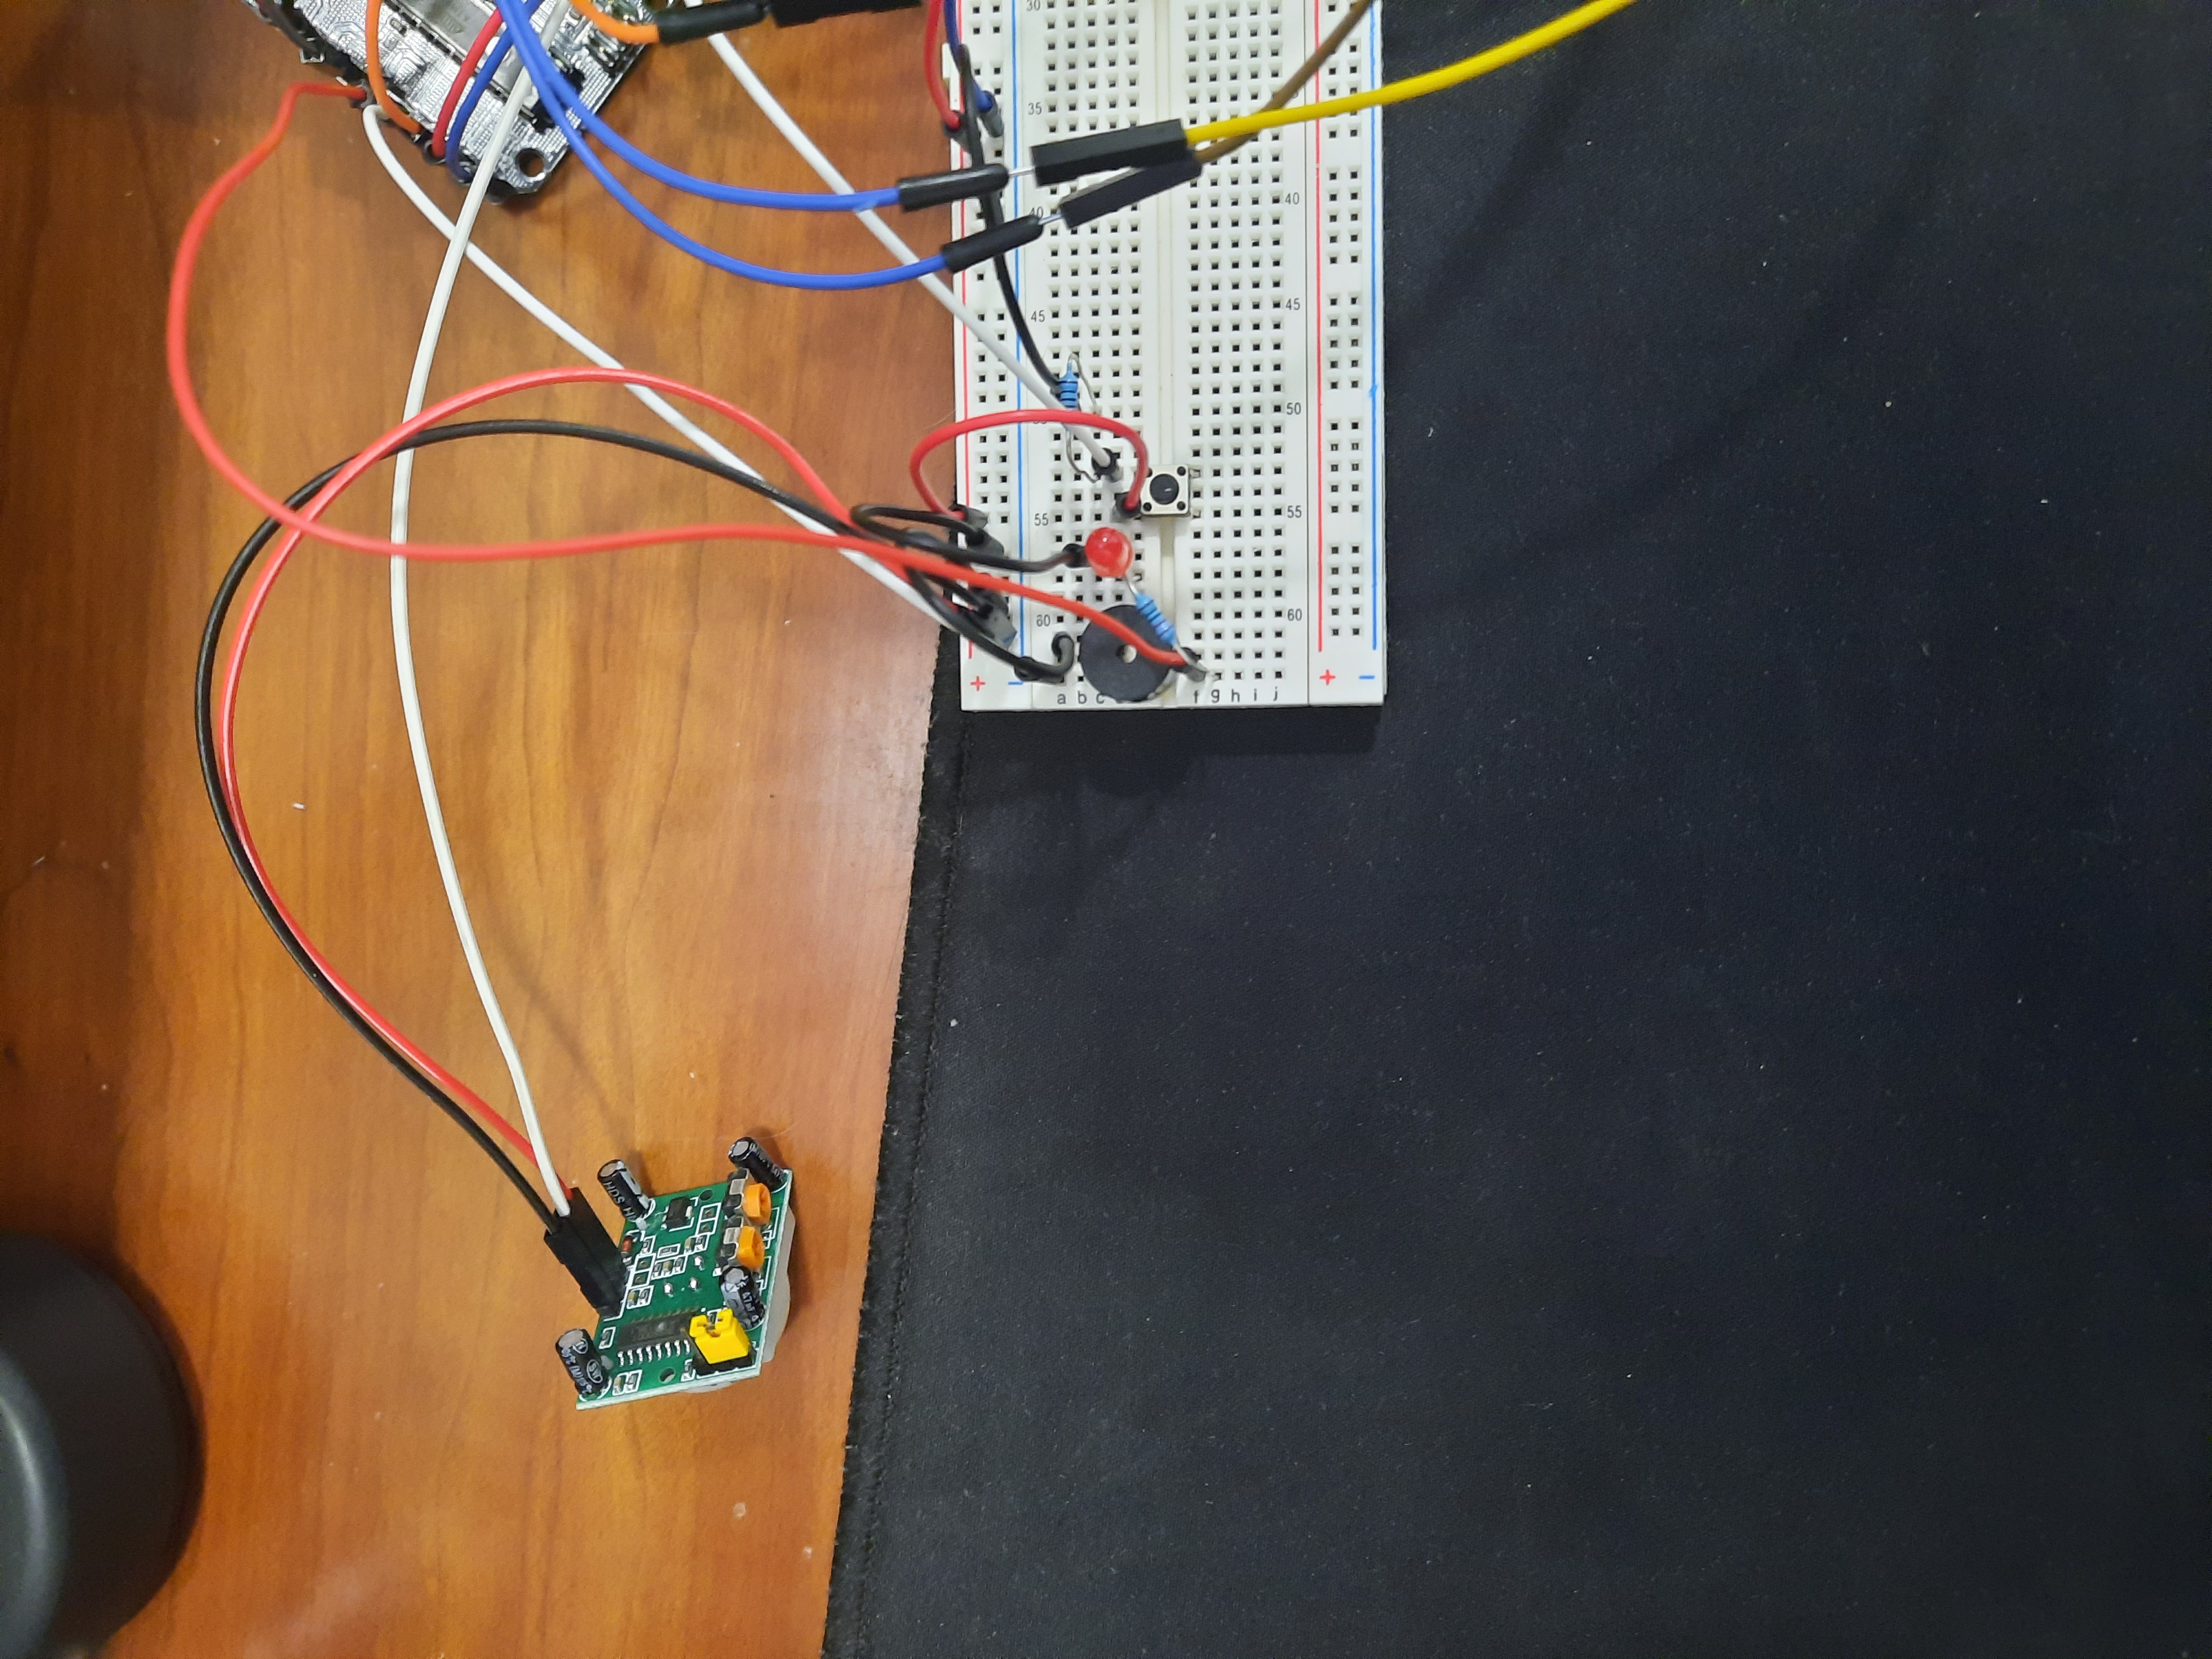
\includegraphics[scale=0.05,angle=-90]{images/testes/sisD_off.jpg}
    \selectlanguage{portuguese}\caption{On vs Off}
\end{figure}